\documentclass[12pt]{article}
\usepackage[none]{hyphenat}
\usepackage{amsmath}
\usepackage{float}
\usepackage{graphicx}
\usepackage{atbegshi}
\AtBeginDocument{\AtBeginShipoutNext{\AtBeginShipoutDiscard}}
\newcommand{\solution}{\noindent \textbf{Solution: }}
\providecommand{\brak}[1]{\ensuremath{\left(#1\right)}}
\newcommand{\myvec}[1]{\ensuremath{\begin{pmatrix}#1\end{pmatrix}}}
\let\vec\mathbf
\begin{document}
\graphicspath{{./Documents}{./figs}}
\begin{center}
  \title{\textbf{Linear Forms}}
  \date{\vspace{-5ex}}
  \maketitle
\end{center}
\setcounter{page}{1}
\section*{11$ ^{th} $ Maths - Chapter 10}
The following problem is question 13 from exercise 10.3:
\begin{enumerate}
  \item Find the equation of the right bisector of the
 line segment joining the points (3, 4) and (–1, 2).
\end{enumerate}
\solution \\
Let \\
\begin{align}
    \overrightarrow{OP} = 3 \hat{i} + 4 \hat{j}
    \label{eq:1}
    \end{align}
    \begin{align}
    \overrightarrow{OQ} = - \hat{i} + 2 \hat{j}
    \label{eq:2}
    \end{align}
    \begin{align}
    \overrightarrow{OR} &= \frac{( 3 - 1 )\hat{i} + (4 + 2)\hat{j}}{2}
    \label{eq:3}
    \end{align}
    \begin{align}
    \overrightarrow{OR} &=\hat{i} + 3 \hat{j}
\end{align}
Slope of the line passing through \eqref{eq:1} and \eqref{eq:2} is\\
given by
\begin{align}
    m_1 &= \frac{2 - 4}{-1 - 3}\\
    &= \frac{-2}{-4}\\
    &= \frac{1}{2}
\end{align}
Slope of the perpendicular line is given by $ m_2 $ = -2
The equation of right bisector passing though \eqref{eq:3} is given by
\begin{align}
    ( y - y_1 ) &= m_2 ( x - x_1 )\\
    ( y - 3 ) &= -2 ( x - 1 )\\
     y - 3 &= - 2x + 2 \\
     2x + y &= 5
\end{align}
\begin{figure}[H]
    \centering
    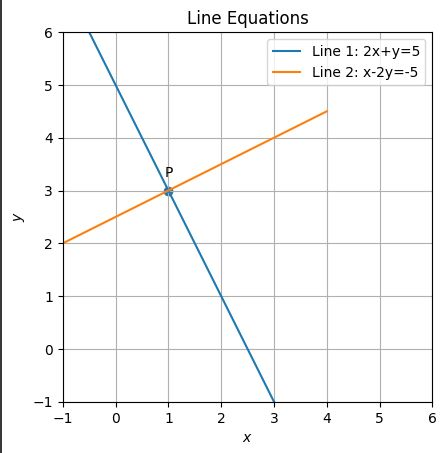
\includegraphics[width=\columnwidth]{figs/graph.jpg}
    \caption{graph}
    \label{fig:}
\end{figure}
\end{document}
